\documentclass{llncs}
\usepackage{multirow}
\usepackage{amsmath,amssymb}
\usepackage{url}
\usepackage{overpic}
\usepackage{enumerate}
\usepackage{graphicx}        % standard LaTeX graphics tool
\usepackage{tikz}        % standard LaTeX graphics tool
\usepackage{subfigure}                                 % authors: subfigures
\usepackage[ruled,vlined,linesnumbered]{algorithm2e}   % authors: last version of algorithm display
\usepackage{todonotes}
\usepackage[ruled,vlined,linesnumbered]{algorithm2e}

%\title{A Subquadratic and Separable Algorithm for Chamfer Norm
  %Distance Transformation \thanks{This work has been mainly funded
  %  by  ANR-11-BS02-009 and  ANR-11-IDEX-0007-02 PALSE/2013/21 research grants.}}


\title{2D Subquadratic Separable Distance Transformation for
  Path-Based Norms\thanks{This work has been mainly funded by
    ANR-11-BS02-009 and ANR-11-IDEX-0007-02 PALSE/2013/21 research
    grants.}}

%% \title{Generic Separable Algorithms for Distance Transformation: A
%%   Subquadratic Approach for Path Based Norms\thanks{This work has been
%%     mainly funded by ANR-11-BS02-009 and ANR-11-IDEX-0007-02
%%     PALSE/2013/21 research grants.}}

\author{David Coeurjolly}

 \institute{ CNRS,  LIRIS, UMR5205, F-69621, France\\
   %\email{david.coeurjolly@liris.cnrs.fr}
}
\graphicspath{{./Figs/}}
%fonts bonanza
\usepackage{amsmath,amssymb,amsfonts}
\usepackage{pifont}% http://ctan.org/pkg/pifont
\newcommand{\CheckMark}{\ding{51}}%
\newcommand{\CrossMark}{\ding{55}}%
% Zapf font
\usepackage[mathscr]{euscript}
\DeclareFontFamily{OT1}{pzc}{}
\DeclareFontShape{OT1}{pzc}{m}{it}%
              {<-> s * [1.2] pzcmi7t}{}
\DeclareMathAlphabet{\mathpzc}{OT1}{pzc}{m}{it}
% rescaling cal to be a touch smaller
\DeclareFontFamily{OMS}{fcmsy}{\skewchar\font48 }
\DeclareFontShape{OMS}{fcmsy}{m}{n}{%
         <-5.5> [.96] cmsy5     <5.5-6.5> [.96] cmsy6
      <6.5-7.5> [.96] cmsy7     <7.5-8.5> [.96] cmsy8
      <8.5-9.5> [.96] cmsy9     <9.5->  [.96] cmsy10
      }{}
\DeclareFontShape{OMS}{fcmsy}{b}{n}{%
       <-6> [.96] cmbsy5
      <6-8> [.96] cmbsy7
      <8->  [.96] cmbsy10
      }{}
\DeclareMathAlphabet{\mathcal}{OMS}{fcmsy}{m}{n}
\usepackage{bbm}

\usepackage{mathtools}% http://ctan.org/pkg/mathtools
\usepackage{calc}% http://ctan.org/pkg/calc

\newcommand*{\mytilde}[2][0pt]{%
  \setbox0=\hbox{$#2$}%
  \tilde{\mathrlap{\phantom{\rule{\wd0}{\ht0+{#1}}}}\smash{#2}}%
}
\newcommand*{\mywidetilde}[2][0pt]{%
  \setbox0=\hbox{$#2$}%
  \widetilde{\mathrlap{\phantom{\rule{\wd0}{\ht0+{#1}}}}\smash{#2}}%
}

%%Space, Lattices
\newcommand{\Z}{{\mathbb{Z}}}
\newcommand{\R}{{\mathbb{R}}}

%%Formulas
\newcommand{\EqDef}{\!\ensuremath{\mathrel{\mathop:}=}\!}
%\newcommand{\EqDef}{\smash{\ensuremath{\stackrel{\text{def}}{=}}}}

%% Misc.
\newcommand{\txtblue}[1]{\textcolor{blue}{ #1}}
\newcommand{\txtgreen}[1]{\textcolor{green}{ #1}}
\newcommand{\txtred}[1]{\textcolor{red}{ #1}}

\begin{document}
\maketitle


\begin{abstract}\sloppy
In many applications, separable algorithms have demonstrated their
efficiency to perform high performance volumetric computations, such
as distance transformation or medial axis extraction. In the
literature, several authors have discussed about the conditions on the
metric to be considered in a separable approach.  In this article, we
present generic separable algorithms to efficiently compute Voronoi
maps and distance transformations for a large class of
metrics. Focusing to path based norms (chamfer masks, neighborhood
sequences, ...), we detail a subquadratic algorithm to compute such
volumetric transformations in dimension 2. More precisely, we describe
a $O(\log^2{m}\cdot N^2)$ algorithm in dimension 2 for shapes in a
$N\times N$ domain with chamfer norm of size $m$.

\keywords{Digital Geometry, Distance Transformation, Path-based Norms}
\end{abstract}

\section{Introduction}
\label{sec:introduction}

Since early works on digital geometry, distance transformation plays
an important role in many applications
\cite{Rosenfeld1966,Rosenfeld1968}. Given a finite input shape
$X\subset \Z^n$, the distance transformation labels each point in $X$
with the distance to its closest point in $\Z^n \setminus X$ (labeling
each point by the closest background point leads to Voronoi maps, see
below). Since such characterization is parametrized by a distance
function, many works have been done to address this distance
transformation problem with a trade-off between algorithmic
performances and the \emph{accuracy} of the digital distance function
with respect to the Euclidean one.  Hence, authors have considered
distances based on chamfer masks
\cite{Rosenfeld1968,borgefors,fouard:ivc:2005} or sequences of chamfer
masks \cite{Rosenfeld1966,mukherjee,Strand2008,DBLP:conf/dgci/NormandSE13};
the vector displacement based Euclidean distance
\cite{danielson,ragnemalm}; the Voronoi diagram based Euclidean
distance \cite{BreuEtAl95,Maurer2003} or the square of the Euclidean
distance \cite{Hirata,roerdnik}.  For Euclidean or $L_p$ metrics,
separable volumetric computations have demonstrated to be very
efficient: optimal $O(n\cdot N^n)$ time algorithms for shapes in $N^n$
domains, optimal multi-thread/GPU implementation\ldots (please refer
to \cite{dcoeurjo_ChapDTWADGMM} for a discussion). For path-based
metrics (chamfer mask, -weighted- neighborhood sequences,\ldots), two
main techniques exist to compute the distance transformation. The
first one considers a weighted graph formulation of the problem, and
shortest path in graphs using Dijkstra-like algorithm can be
considered. If $m$ denotes the size of the chamfer mask, computational
cost could be in $O(m\cdot N^n)$ using a cyclic bucket data structure
\cite{verwer_uniform}. Another approach consists in a raster scan of
the domain: first the chamfer mask is decomposed into two disjoint
sub-masks. Then the domain grid points are scanned in a given order
(consistent with the sub-masks construction) and a local minimum
computation is performed and then propagated
\cite{Rosenfeld1966,borgefors}. Scanning the domain twice for each
sub-masks leads to the distance transformation. Again, we end up with
a $O(m\cdot N^n)$ computational cost. This complexity is said to be
quadratic in $m$ and $N$ since for arbitrary large image $N$, even if
$m \ll N$, $m$ has to be in $O(N^n)$ to have accurate asymptotic DT.
Please note that Dijkstra's graph approach allows us to defined
constrained distance transformation (\emph{i.e.} geodesic metric),
both separable approaches and raster-scan for path-based metrics are
only dedicated to compact convex domains (usually hyper-rectangular)
distance transformation.


\textbf{Contributions} In this article, we first describe the generic
framework for separable distance transformation and conditions on the
metric to be consistent with this model. Then, we describe
subquadratic algorithms in dimension 2 to compute error-free distance
transformation and Voronoi map for chamfer norms and other path-based
metrics. Overall computational costs can be summarized as follows:
%\begin{table}
%  \caption{Computational cost summary for separable Voronoi map
%    computation on $N^n$ domains ($m$ being the size of the chamfer
%    norm and $f$ the number of row in a H-representation, see below).}
 % \label{tab:final}
  \begin{center}
    \begin{tabular}{|c|c|c|c|c|}
      \hline
      Metric &\textsc{Closest}& \textsc{HiddenBy} & Sep. Voronoi Map & Reference\\
      \hline
      $L_2$ & $O(1)$ &  $O(1)$ & $\Theta(n\cdot N^n)$ & \cite{Hirata}\\
      $L_\infty$ & $O(1)$ & $O(1)$ &  $\Theta(n\cdot N^n)$ & \cite{roerdnik}\\
      $L_1$ & $O(1)$ &   $O(1)$ &$\Theta(n\cdot N^n)$& \cite{roerdnik}\\
      $L_p$  (exact pred.) & $O(\log{p})$ &
      $O(\log{p}\cdot\log{N})$ & $O(n\cdot
      N^n\cdot\log{p}\cdot\log{N})$& Lem.~\ref{lem:generic},  \cite{dgtal}\\
      $L_p$  (inexact pred.) & $O(1)$ &
      $O(\log{N})$ & $O(n\cdot
      N^n\cdot\log{N})$& Lem.~\ref{lem:generic},  \cite{dgtal}\\
      2D Chamfer norm &  $O(\log{m})$ &$O(\log^2{m})$
      &$O(\log^2{m}\cdot N^2)$& Theorem \ref{them}\\
  %    3D Chamfer norm &  $O(\log{m})$ &$O(\log^2{m})$
  %    &$O(\log^2{m}\cdot N^3)$& Theorem \ref{them2}\\
  %    nD Chamfer norm &  $O(n\cdot\log{f})$ &$O(n\cdot log^2{f}\cdot\log{N})$
  %    & $O(n^2\cdot N^n\cdot \log{f}\cdot\log{N})$& Corollary \ref{coro2}\\
      2D Neig. seq. norm  & $O(\log{f})$&
      $O(\log^2{f})$& $O(\log^2{}f\cdot N^2)$& Th.~\ref{them} and  \cite{DBLP:conf/dgci/NormandSE13}\\
      \hline
    \end{tabular}
  \end{center}
%\end{table}
\section{Preliminaries}
\label{sec:preliminaries}
%% Let us first define some elementary concepts and objects.
%% \begin{definition}[Metrics and Metric Space]
%%   \label{def:distance}
%%   A metric is a map $d$ from $E$ to a sub-group $F$ of $\R$ such that
%%   $\forall a,b,c\in E$,
%%   \begin{align}
%%     (\text{non-negative})\quad & d(a,b)\geq 0\\
%%     (\text{identity of indiscernibles}) \quad&  d(a,b)= 0
%%     \Leftrightarrow a=b\\
%%     (\text{symmetry})\quad &  d(a,b)=d(b,a)\\
%%     (\text{triangular inequality})\quad &   d(a,c) \leq d(a,b) + d(b,c)
%%   \end{align}
%% $(E, F, d)$ is called a metric space.
%% \end{definition}
%% If property $(4)$ is omitted, we are defining a distance function
%% instead of a metric.
\begin{definition}[Norm and metric induced by a norm]
  \label{def:norm}
  Given a vector space EV, a norm is a map $g$ from  $EV$ to a sub-group
  $F$ of $\R$ such that $\forall \vec{x},\vec{y}\in EV$,
  \begin{align}
    (\text{non-negative})\quad & g(\vec{x})\geq 0\\
    (\text{identity of indiscernibles}) \quad&  g(\vec{x})= 0
    \Leftrightarrow \vec{x}=\vec{0}\\
    (\text{triangular inequality})\quad &   g(\vec{x}+\vec{y}) \leq
    g(\vec{x}) + g(\vec{y})\\
    (\text{homogeneity})\quad &  \forall \lambda\in\R, \quad
    g(\lambda\cdot\vec{x}) = |\lambda|\cdot g(\cdot\vec{x})
  \end{align}
$d(a,b) \EqDef g(b-a)$ is the metric induced by the
  norm $g$.  $(E, F, d)$ is called a  metric space if $d:~E\rightarrow
  F$.
\end{definition}
Note that the above definition can be extended from vector spaces to
\emph{modules} on a commutative ring ($\Z^n$ being a module on $\Z$
but not a vector space) \cite{Thiel_hdr}. Path-based approaches
(chamfer masks, -weighted- neighborhood sequences...)  aim at defining
metrics induced by norms in metric spaces $(\Z^n, \Z , d)$.  Note that
(weighed, with $w_i\geq 0$) $L_p$ metrics
\begin{equation}
    d_{L_p} (a,b) = \left ( \sum_{k=1}^n w_k|a_k-b_k |^p \right )^{\frac{1}{p}}\;,
  \end{equation}
characterize metric spaces $(\Z^n, \R , d_{L_p})$. Rounding the \sloppy
distance function $(\Z^n,\Z, \lceil d_{L_p}\rceil)$ is a metric
space \cite{klette_book}.

\begin{definition}[Distance Transformation and Voronoi Map]
  The distance transform $DT_X$ associated with a digital metric space
  $(\Z^n,\Z,d)$ is a map  $X\rightarrow\Z$ such that, for $a\in X$
  $    DT_X(a) = \min_{b\in \Z^n\setminus X} \{d(a,b)\}$.
The Voronoi map is the map $X\rightarrow\Z^n$:
$    \Pi_X(a) = \argmin_{b\in \Z^n\setminus X} \{d(a,b)\}$.
\end{definition}
Voronoi map $\Pi_X$ corresponds to the intersection between the
continuous Voronoi diagram for the metric $d$ of points
$\Z^n\setminus$ and the lattice $\Z^n$. If a digital point $a$ belongs
to a Voronoi diagram $d-$facet ($1\leq d< n$), $a$ is equidistant to 2
or more points in $\Z^n\setminus X$ but only one is considered in
$\Pi_X(a)$ this choice has no influence on $DT_X$.
% (please refer to \cite{Couprie2007} for complete digital
%Voronoi map).
\begin{definition}[Chamfer Mask]
  A weighted vector is a pair $(\vec{v},w)$ with $\vec{v}\in\Z^n$ and
  $w\in\N^*$. A chamfer mask $\M$ is a central-symmetric set of weighted
  vectors with non-empty vectors and containing at least a basis of
  $\Z^n$.
\end{definition}
Many authors have proposed algorithmic and/or analytic approaches to
construct chamfer masks approximating the Euclidean metric and being
induced by a norm. In the following, we focus on such \emph{chamfer
  norms}.  To evaluate distances between two digital points for a
given chamfer metric, direct formulations have been proposed with
simple geometrical interpretation:
\begin{definition}[Rational ball, minimal H-representation \cite{Thiel_hdr,DBLP:journals/pr/NormandE09}]
  Given a Chamfer mask $\M$ inducing a norm, the rational ball
  associated with $\M$ is the polytope
  \begin{equation}
\label{eq:4}
    \B = conv\left\{ \frac{\vec{v}_k}{w_k};\; (\vec{v}_k,w_k)\in\M \right \}\,.
  \end{equation}
Rational ball $\B$ can also be described in a H-representation of
polytope with minimal parameter \cite{DBLP:conf/dgci/NormandSE13}: $ P
= \{ x\in\Z^n; Ax \leq y\;\}$ such that $\forall k\in[1\ldots f],
~\exists x\in P\quad A_kx=y_k.\footnote{$A_k$ being the $k^{th}$ row
  of $A$.}$ $f$ being the number of row in $A$ and the number of
facets in $\B$, and is thus related to $|\M|$.
\end{definition}
An important result for distance computation can be formalized as follows:
\begin{proposition}[Direct Distance Computation \cite{DBLP:journals/pr/NormandE09}]
  Given a chamfer mask $\M$ induced by a  norm and $(A,y)$ its minimal
  parameter H-representation, then for any $a\in\Z^n$, the chamfer
  distance of $a$ from the origin is
  \begin{equation}
    \label{eq:1}
    d_\M(O,a) =  \max_{1\leq k \leq f} \{ A_k a^T\}\,.
  \end{equation}
\end{proposition}
Among path-based digital metric, we can also introduce (weighted)
neighborhood sequences
\cite{Rosenfeld1966,mukherjee,Strand2008,DBLP:conf/dgci/NormandSE13}
whose objective is to have better approximation of the Euclidean
metric from sequences of elementary chamfer masks.  A key result have
been demonstrated in \cite{DBLP:conf/dgci/NormandSE13} stating that
for such distance functions, a minimal parameter polytope
representation exists and that distances can be obtained from similar
expression to (\ref{eq:1}):
\begin{equation}
  d(O,a)  =\max_{1\leq k \leq f} \{ f_k(A_k a^T)\}\,,
\end{equation}
$f_k$ being some integer sequence characterizing the neighborhood
sequence metric. In the following and for the sake of simplicity, we
describe our algorithms focusing on chamfer norms but similar results
can be obtained for more generic path-based metric such as
neighborhood sequences.
\section{Separable Distance Transformation}
\label{sec:separ-dist-transf}
\subsection{Voronoi Map from Separable Approach and Metric Conditions}
\label{sec:voronoi-map-from}
In \cite{Hirata,BreuEtAl95,roerdnik,Maurer2003},
several authors have described optimal in time and separable
techniques to compute error-free Voronoi maps or distance
transformations for $L_2$ and $L_p$ metrics. Separability means that
computations are performed dimension by dimension
%, allowing fast
%computations and multithread implementations (see
%\cite{dcoeurjo_ChapDT} for an overview).
In the following, we
consider Voronoi map approach as defined in \cite{BreuEtAl95}: Let us
first define hyper-rectangular image $I_X:
[1..N_1]\times\ldots\times[1..N_n] \rightarrow \{0,1\}$ such that $X\subset
I_X$ and $I_X(a)= 1$ for $a\in [1..N_1]\times\ldots\times[1..N_n]$ iff $a\in
X$ ($I_X(a)=0$ otherwise). In dimension 2, we first process each row
of the input image to create independent 1D Voronoi maps along the
first dimension for the metric. Then, for each further dimension, the
partial Voronoi map $\Pi_X$ is updated using one dimensional
independent processes on image spans along the $i^{th}$ dimension.
%% \begin{figure}
%%   \begin{center}
%%      \begin{overpic}[draft=false,width=10cm]{figs/edt_dcoeurjo}
%%        \put(30,5){$Candidates_S$}
%%        \put(57,0){$S$}
%%      \end{overpic}
%%   \end{center}
%%   \caption{Voronoi Map construction in dimension 2.\label{fig:2Dbreu}}
%% \end{figure}
Algorithm \ref{alg:voro} describes the 1D processes to perform on each
row, column and higher dimensional image span\footnote{An image span
  $S$ along the $i^{th}$ direction is a vector of $N_i$ points with
  same coordinates except at $i$.} In this process, metric information
are embedded in the following two predicates (see
Fig.~\ref{fig:predicates}): \textsc{Closest}$(a, b, c)$, given three
points $a,b,c\in\Z^n$ this predicate returns true if $d(a,b) <
d(a,c)$. \textsc{HiddenBy}$(a, b, c, S)$, given three points
$a,b,c\in\Z^n$ such that $a_i<b_i<c_i$ and a 1D image span
$S$\footnote{Subscript $a_i$ denotes the $i^{th}$ coordinate of point
  $a\in\Z^n$.}, this
predicates returns true if there is no $s\in S$ such that
    \begin{equation}
      d(b,s) < d(a,s)\text{ and }  d(b,s) < d(c,s)\,.
    \end{equation}
\begin{algorithm}[H]\footnotesize
  \KwData{Input binary map $I_X$ if $i=1$ or  partial Voronoi map $\Pi_X$ obtained for
    dimensions lower than $i$, and a 1D span $S$ with points
    $\{s^1,\ldots,s^{N_i}\}$ sorted by their $i^{th}$ coordinate.}
  \KwResult{Updated partial Voronoi map $\Pi_X$ along $S$.}
\If{ i = 1}
{ $k=0$\;
\ForEach{point $s$ in $S$}{
    \If{$I_X(s) = 1$}
     {
       $L_S[k] = s$\;
       $k++$\;
     }
}
}
\Else{
 ${L}_S[0]=\Pi_X(s^1)$\;
  ${L}_S[1]=\Pi_X(s^2)$\;
  $k=2$ , $l=3$\;
  \While{$l\leq N_i$}{
    $w = \Pi_X(s^l)$\;
    \While{$k\geq 2$ and \textsc{HiddenBy}(${L}_S[k-1],{L}_S[k],w, S$)}
          {
         $ k--$\;
        }
        $k++$ ; $l++$\;
        ${L}_S[k]=w$\;
  }
}
  \ForEach{point  $s$ in $S$ by increasing $i^{th}$ coordinate}
  {
    \While{($k < |L_S|$) and not(\textsc{Closest}($s^i$, $L_S[k]$, $L_S[k+1]$))}
          {
            $k++$\;
          }
    $\Pi_X[s] = L_S[k]$\;
  }

  \caption{Voronoi map construction on 1D image span $S$ along the
    $i^{th}$ dimension.\label{alg:voro}}
\end{algorithm}
\begin{figure}
  \begin{center}
    \subfigure[]{ \begin{overpic}[width=2cm]{figs/hiddenByTrue}
    \put(26,5){$a$}
    \put(0,35){$b$}
    \put(25,75){$c$}
    \put(55,-15){$S$}
    \end{overpic}}
    \subfigure[]{\begin{overpic}[width=2cm]{figs/hiddenByFalse}
    \put(37,8){$a$}
    \put(23,37){$b$}
    \put(30,72){$c$}
    \put(55,-15){$S$}
    \end{overpic}}~~~~~~~~~~
    \subfigure[]{\begin{overpic}[width=1.1cm]{figs/closest}
    \put(-5,52){$a$}
    \put(2,78){$b$}
    \put(47,55){$c$}
    \put(38,-15){$S$}
      \end{overpic}
    }
  \end{center}
  \caption{\small Geometrical predicates for Voronoi map construction:
    \textsc{HiddenBy}($a,b,c,S)$ returns false in $(a)$ and true in
    $(b)$ (straight segments correspond to Voronoi diagram
    edges). $(c)$ illustrates the \textsc{Closest}($a,b,c$) predicate
    for $c\in S$.}
  \label{fig:predicates}
\end{figure}


In other words, \textsc{HiddenBy} returns true if and only if the
Voronoi cell of sites $a$ and $c$ \emph{hide} the Voronoi cell of $b$
along $S$.  For $L_1$, $L_2$ and $L_\infty$ metrics,
\textsc{Closest} and \textsc{HiddenBy} predicates can be computed in
$O(1)$ \cite{BreuEtAl95,Hirata,roerdnik}. Hence, Algorithm
\ref{alg:voro} is in $O(N_i)$ for dimension $i$, leading to an overall
computational time for the Voronoi map and distance transformation
problem in $\Theta(n\cdot N^n)$ (if we assume that $\forall i\in[1\ldots
  n], N_i=N$).

In \cite{Hirata} or \cite{Maurer2003}, authors discussed about
conditions on the metric $d$ to ensure that Algorithm \ref{alg:voro}
is correct. The key property can be informally describe as follows:
given two points $a,b\in\Z^n$ such that $a_i<b_i$ and a straight line
$l$ along the $i^{th}$ direction and if we denote by $v_l(a)$
(resp. $v_l(b)$) the intersection between the Voronoi cell of $a$
(resp. $b$) and l, then $v_l(a)$ and $v_l(b)$ are simply connected
Euclidean segments and $v_l(a)$ appears \emph{before} $v_l(b)$ on $l$
(so called \emph{monotonicity property} in \cite{Maurer2003} and is
related to \emph{quadrangle inequality} in \cite{Hirata}).  To sum
up these contributions, we have the following proposition:
\begin{proposition}[Metric conditions \cite{Hirata}]
\label{prop:voronoi-map-from-1}
  Let $d$ be a metric induced by a \textbf{norm whose unit ball is
    symmetric with respect to grid axes} and if distance comparison
  predicate is exact, Algorithm 1 is correct and returns a Voronoi map
  $\Pi_X$.
\end{proposition}
When implementing Algorithm 1, we say that the distance comparison
predicate is exact if we can compare two distances, \emph{e.g.}
\textsc{Closest} predicate, without error. Hence, Algorithm \ref{alg:voro}
provides exact Voronoi map computation for $L_p$ norms. In this case,
distance comparison predicate can be implemented error-free from
integer number comparison considering the $p$ power of the distance
function $\left (d_{L_p}\right)^p$.  Proposition
\ref{prop:voronoi-map-from-1} also implies that most chamfer norms and
neighborhood sequences based norms can also be considered in separable
Algorithm \ref{alg:voro} (see Fig.~\ref{fig:metrics}). We just need
algorithmic tools to efficiently implement both \textsc{Closest} and
\textsc{HiddenBy} predicates.
\begin{figure}[htbp]
 {
\includegraphics[width=1.65cm]{image-ball-1}}
 {
\includegraphics[width=1.65cm]{image-ball-1-4}}
 {
\includegraphics[width=1.65cm]{image-ball-2}}
 {
\includegraphics[width=1.65cm]{image-ball-4}}
 {
\includegraphics[width=1.65cm]{image-ball-43-1}}
 {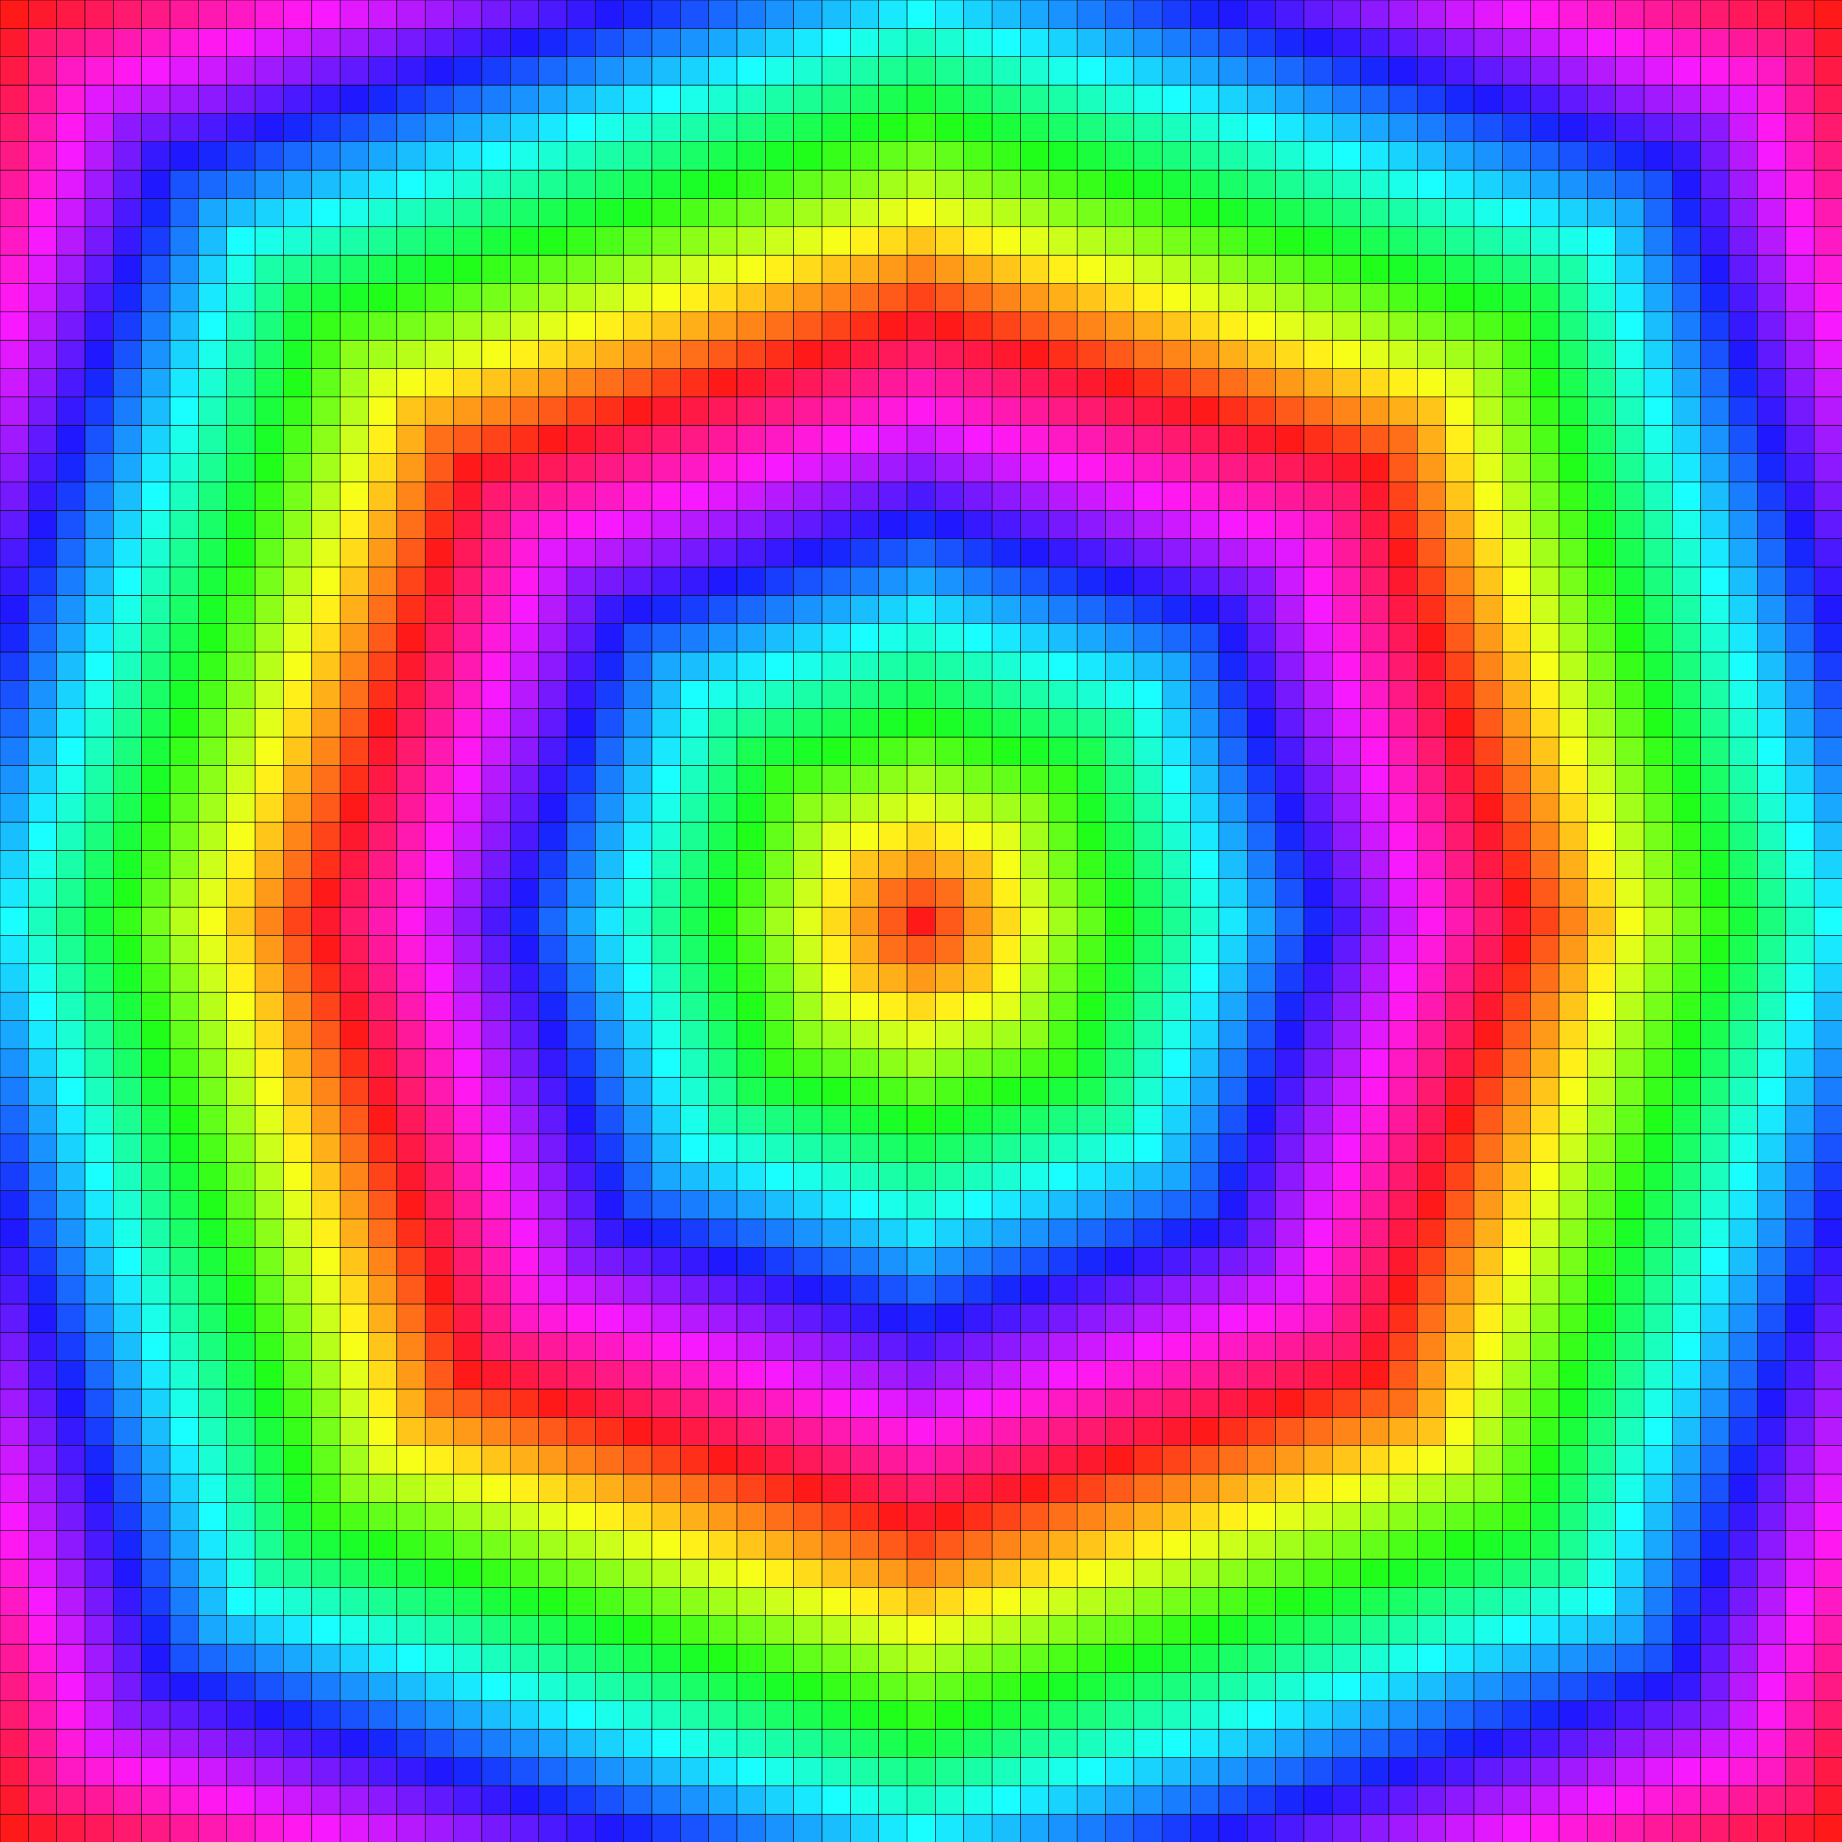
\includegraphics[width=1.65cm]{image-ball-chamf34}}
 {
\includegraphics[width=1.65cm]{image-ball-chamf5711}}
  \caption{Balls for different metrics satisfying Proposition \ref{prop:voronoi-map-from-1}: \emph{(from
      left to right)} $L_1$, $L_{1.4}$, $L_2$, $L_4$, $L_{43.1}$,
    $\M_{3-4}$ and $\M_{5-7-11}$.}
  \label{fig:metrics}
\end{figure}
%
\vspace{-1cm}
\subsection{A First Generic Adapter}
\label{sec:first-gener-adapt}
We first detail the overall computational cost of Algorithm
\ref{alg:voro}:
\begin{lemma}
\label{lem:generic}
Let $(\Z^n, F, d)$ be a metric space induced by a norm with axis
symmetric unit ball. If $C$ denotes the computational cost of
\textsc{Closest} predicate and $H$ is the computational cost of the
\textsc{HiddenBy} predicate, then Algorithm \ref{alg:voro} is in
$O(n\cdot N^n\cdot (C+H))$.
\end{lemma}
From \cite{BreuEtAl95,roerdnik}, $C=H=O(1)$ for $L_1,L_2$ and $L_\infty$
norms.  For prescribed norm $d$, we first define generic
Algorithms~\ref{alg:genclosest}, \ref{alg:genedge} and
\ref{alg:genhidden}: from some evaluations of $d$, \textsc{HiddenBy}
predicate is obtained by a dichotomic search on the 1D image span $S$
to localize the abscissa of Voronoi edges of sites $\{a,b\}$ and
$\{b,c\}$ (see Fig.~\ref{fig:algo}).

\begin{algorithm}[H]\footnotesize
  \Return $d(a,b) < d(a,c)$\;
  \caption{\footnotesize Generic \textsc{Closest}($a,b,c\in\Z^n$).\label{alg:genclosest}}
\end{algorithm}

\begin{algorithm}[H]\footnotesize
  \If{$(j-i=1)$}
     {
       \If{$i=1$ and \textsc{Closest}$(s^{i},b,a)$ }{\Return $-\infty$\;}
       \If{$i=N_i$ and \textsc{Closest}$(s^{i},a,b)$ }{\Return $\infty$\;}
       \Return  i\;
     }
     $mid  = i + (j-i)/2$\;
     \eIf{\textsc{Closest}$(s^{mid},a,b)$}
       {
         \tcp{$s_{mid}$ closer to $a$}
         \Return \textsc{VoronoiEdge}($a,b,s^{mid},s^j$)
}
 {
         \tcp{$s_{mid}$ closer to $b$}
         \Return \textsc{VoronoiEdge}($a,b,s^{i},s^{mid}$)
}

  \caption{\footnotesize Generic \textsc{VoronoiEdge}($a,b,s^i,s^j\in\Z^n$), $a_i<b_i$.\label{alg:genedge}}
\end{algorithm}

\begin{algorithm}[H]\footnotesize
  $v_{ab}$ = \textsc{VoronoiEdge}$(a,b,s^1, s^{N_i})$\;
  $v_{bc}$ = \textsc{VoronoiEdge}$(b,c,s^1, s^{N_i})$\;
  \Return $(v_{ab}> v_{bc})$\;
  \caption{\footnotesize Generic \textsc{HiddenBy}($a,b,c\in\Z^n; S$ in the $i^{th}$
    direction) $a_i<b_i<c_i$.\label{alg:genhidden}}
\end{algorithm}
\begin{lemma}
\label{lem:genericDich}
   Let $(\Z^n, F, d)$ be a metric space induced by a norm with axis
   symmetric unit ball,   from Algorithms \ref{alg:genclosest} and
   \ref{alg:genhidden}, we have $H=O(C\cdot \log{N})$.
\end{lemma}
\begin{proof}
  First, the generic \textsc{VoronoiEdge} is dichotomic in
  $O(\log{N})$ steps and $O(C)$ for each one. \textsc{VoronoiEdge} is
  in $O(C\cdot\log{N})$.  To prove the correctness of
  \textsc{VoronoiEdge} (and thus Alg.~\ref{alg:voro}), we use the
  convexity of the metric and the quadrangle property: since
  $a_i<b_i$, all grid points closer to $a$ than $b$ in $S$ (if exist)
  are \emph{lower} than all pixels on $S$ closer to $b$ than to $a$
  (if exist too). Thanks to test in line $4$, recursive call maintain
  this invariant. Note that tests $2-5$ handle the fact that the edge
  may not belong to $S$.$\Box$
\end{proof}
If we consider a chamfer norm with $f$ facet rational ball, Eq.~(\ref{eq:1})
suggests that $C=O(f)$. Hence, we have the following corollary:
\begin{corollary}
  Let $\M$ be a chamfer norm whose rational ball has $f$ facets,
  separable exact Voronoi map $\Pi_X$ can be obtained in
    $O(n\cdot N^n\cdot f \cdot \log{N})$.
\end{corollary}
Please remember that naive implementation of chamfer mask distance
transformation using raster scan approach would lead to a $O(f\cdot
N^n)$ computational cost. In the following sections, we use the convex
structure of $\B$ to design a first subquadratic algorithm for chamfer
norms.

\subsection{Subquadratic Algorithm in Dimension 2}
\label{sec:subq-algor-dimens}

Let us consider a 2D chamfer norm $\M$ with $m$ weighted vectors (note
that $f\EqDef|\B| = m$ in 2D). We suppose that vectors
$\{\vec{v}^k\}_{k=1\ldots m}$ are sorted counterclockwise. We define a wedge
as a pair $(\vec{v}^k,\vec{v}^{k+1})$ of vectors. To each wedge is
associated a row $A_k$ in the minimal H-representation of $A$ ($A_k$
can also be seen as a  --non-unitary-- normal vectors to $\B$ facets
\cite{DBLP:journals/pr/NormandE09}). Using similar notations,
\cite{Thiel_hdr,Strand2008} demonstrate that the distance evaluation
of point $a$ can be obtained in two steps: First, we compute the wedge
$(\vec{v}^k,\vec{v}^{k+1})$, $a$ belongs to. Then,
\begin{equation}
\label{eq:2}
  d_\M(O,a) = A_k\cdot a^T
\end{equation}

\begin{lemma}
\label{lem:log}
  Given a chamfer norm $\M$ in dimension 2 with $m$ vectors, the distance computation
  and thus the \textsc{Closest} predicate are in $O(\log{m})$.
\end{lemma}
\begin{proof}
  Since vectors are sorted counter-clockwise,
  $(\vec{v}^k,\vec{v}^{k+1})$ wedge can be obtained by a dichotomic
  search with $O(\log{m})$ steps. At each step, we compute the local
  orientation of point $a$ w.r.t. a direction which is in $O(1)$. Once
  the wedge has been obtained, Eq.~(\ref{eq:2}) returns the distance
  value in $O(1)$.$\Box$
\end{proof}

Please note that in practical implementations, we can use symmetries
in $\M$ vectors to only work on restrictions of chamfer mask
directions.  To optimize the \textsc{HiddenBy} predicate, we focus on
the \textsc{VoronoiEdge} function. Given two points $a$ and $b$
($a_i<b_i$) and a 1D image span $S$ along the $i^{th}$ dimension, we
have to find the lowest abscissa $e_i$ of the point $e$ on $S$ such
that $d(a,e) < d(b,e)$ and $d(a,e')\geq d(b, e')$ for any $e'$ with
$e'_i>e_i$.
Let us first suppose that we don't have $e$ but we know the two wedges
$(\vec{v}^{k},\vec{v}^{k+1})$ (resp. $(\vec{v}^j,\vec{v}^{j+1})$) such
that the vector $(e-a)^T$ (resp. $(e-b)^T$) belongs to (see
Fig.~\ref{fig:algo}). In this situation, we know that $e$ is the
solution of
\begin{equation}
\label{eq:3}
  A_k\cdot  (e-a)^T = A_j\cdot (e -b)^T\;.
\end{equation}
(since $e\in S$, we have one linear equation with only one unknown
$e_i$). As a consequence, if we know the two wedges the Voronoi edge
belongs to, we have the abscissa in $O(1)$ (see Algorithm
\ref{alg:chamedge} and Fig.~\ref{fig:algo}$-(c)$).
\begin{algorithm}[h]\footnotesize
  $(\vec{v}^k,\vec{v}^{k+1})$ = \textsc{VoronoiEdgeWedge}$(a,b,\vec{v}^1,\vec{v}^m, S)$\;
  $(\vec{v}^j,\vec{v}^{j+1})$ = \textsc{VoronoiEdgeWedge}$(b,a,\vec{v}^1,\vec{v}^m, S)$\;

  Compute the abscissa $e_i$ of the point $e$ such that $A_k\cdot
  (e-a)^T = A_j\cdot (e -b)^T$\;

  \Return $e_i$\;
  \caption{\footnotesize
2D chamfer norm \textsc{VoronoiEdge}($a,b,s^i,s^j\in\Z^2$).\label{alg:chamedge}}
\end{algorithm}
To obtain both wedges, we use a dichotomic search similar to
Algorithm~\ref{alg:genedge}: Algorithm~\ref{alg:chamedgew} returns the
wedge associated with $a$ containing the Voronoi edge with respect to
$b$. Applying this algorithm to obtain the wedge associated with $b$ with respect to
$a$ gives exactly  Algorithm \ref{alg:chamedge}.
\begin{figure}[h]
  \begin{center}\scriptsize
    \subfigure[]{
      \begin{overpic}[width=2.5cm]{init}
        \put(-5,60){$a$}
        \put(85,40){$b$}
        \put(42,105){$S$}
      \end{overpic}
    }~~~~~~~~~
    \subfigure[]{
      \begin{overpic}[width=2.5cm]{algoMid}
      \put(-5,60){$a$}
        \put(85,40){$b$}
        \put(42,105){$S$}
        \put(12,60){$\vec{\vec{v}^{mid}}$}
        \put(13,80){$\vec{\vec{v}^{mid+1}}$}
        \put(-5,98){$\vec{\vec{v}^j}$}
        \put(5,32){$\vec{\vec{v}^i}$}
        \put(50,90){$p^{mid+1}$}
        \put(50,58){$p^{mid}$}
      \end{overpic}
    }~~~~~~~~~
    \subfigure[]{
      \begin{overpic}[width=2.5cm]{algoEnd}
      \put(-5,60){$a$}
        \put(85,40){$b$}
        \put(42,105){$S$}
        \put(50,50){$e$}
        \put(7,45){$\vec{\vec{v}^{k}}$}
        \put(11,70){$\vec{\vec{v}^{k+1}}$}
        \put(60,40){$\vec{\vec{v}^j}$}
        \put(67,57){$\vec{\vec{v}^{j+1}}$}
      \end{overpic}
    }
  \end{center}
  \caption{\small \textsc{VoronoiEdgeWedge} and \textsc{VoronoiEdge}: $(a)$
    initial problem, we want to compute the intersection between $S$
    and the Voronoi edge of $a$ and $b$. $(b)$ an internal step of
    \textsc{VoronoiEdgeWedge} to reduce the set of directions of $\M$
    at $a$ (here the next recursive call will be on
    $(\vec{v}^i,\vec{v}^{mid})$).$(c)$ final step of
    \textsc{VoronoiEdge} where both wedges have been obtained and thus
    $e$ can be computed.}
  \label{fig:algo}
\end{figure}
The dichotomic search shrinks the set of vectors
$\{\vec{v}^i,\ldots,\vec{v}^j\}$ to end up with a wedge
$(\vec{v}^k,\vec{v}^{k+1})$ such that the intersection point between
the straight line $(a + \vec{v}^k)$ and $S$ is in the Voronoi cell of
$a$ and such that the intersection between $(a + \vec{v}^k)$ and $S$
is in the Voronoi cell of $b$ (see
Fig.~\ref{fig:algo}$-(c)$). Algorithm~\ref{alg:chamedgew} thus first
compute the intersection points associated with a wedge
$(\vec{v}^{i+(j-i)/2}, \vec{v}^{i+(j-i)/2+1})$ (lines $5-6$);
Evaluates the distances at these points (lines $7-8$) and then decides
which set $\{\vec{v}^i,\ldots,\vec{v}^{i+(j-i)/2}\}$ or
$\{\vec{v}^{i+(j-i)/2},\ldots,\vec{v}^j\}$ has to be considered for
the recursive call (lines $14-25$ and Fig.~\ref{fig:algo}$-(b)$).

\begin{algorithm}[t]
\footnotesize
  \eIf{ $(j-i =1)$}{
    \Return $(\vec{v}^i,\vec{v}^{i+1})$\;}
{
   $mid  = i + (j-i)/2$\;
   Let $p^{mid}$  be the intersection point between $(a +
   \vec{v}^{mid})$ and $S$\;
  Let $p^{mid+1}$  be the intersection point between $(a +
   \vec{v}^{mid+1})$ and $S$\;


   \tcp*[f]{$O(1)$ evaluation of distances w.r.t. $a$}
   $d^a_{p^{mid}} = A_{mid}\cdot (p^{mid}-e)^T$\;
   $d^a_{p^{mid+1}} = A_{mid+1}\cdot (p^{mid+1}-e)^T$\;


   \tcp*[f]{$O(\log{m})$ evaluation of distances w.r.t. $b$}
   $d^b_{p^{mid}} = d_\M(b, p^{mid})$\;
   $d^b_{p^{mid+1}} = d_\M(b,p^{mid+1})$\;

   Let $b_{mid}$ be true if $d^a_{p^{mid}} < d^b_{p^{mid}}$; false otherwise\;
   Let $b_{mid+1}$ be true if $d^a_{p^{mid+1}} < d^b_{p^{mid+1}}$; false otherwise\;


   \If{ $b_{mid}\neq b_{mid+1}$ \tcp*[r]{we have the Voronoi edge
       wedge}} { \Return $(\vec{v}^{mid},\vec{v}^{mid+1})$\; }

    \If{ $b_{mid}=b_{mid+1}=true$ \tcp*[r]{Both points are in $a$'s cell}}
{
    \eIf{$a_i < b_i$}
{
  \Return \textsc{VoronoiEdgeWedge}$(a,b,\vec{v}^{mid}, \vec{v}^{j}, S)$\;
}
{
  \Return \textsc{VoronoiEdgeWedge}$(a,b,\vec{v}^{i}, \vec{v}^{mid}, S)$\;
}

}
    \If{ $b_{mid}= b_{mid+1}=false$\tcp*[r]{Both points are in $b$'s cell}}
{
    \eIf{$a_i < b_i$}
{
  \Return \textsc{VoronoiEdgeWedge}$(a,b,\vec{v}^{i}, \vec{v}^{mid}, S)$\;
}
{
  \Return \textsc{VoronoiEdgeWedge}$(a,b,\vec{v}^{mid}, \vec{v}^{j}, S)$\;
}

}

}
  \caption{\footnotesize
\textsc{VoronoiEdgeWedge}($a,b\in\Z^2; \vec{v}^i,\vec{v}^j$
    in $\M$; $S$ along the $i^{th}$ direction).\label{alg:chamedgew}}
\end{algorithm}
\begin{theorem}
\label{them}
  Let $\M$ be a 2D chamfer norm with axis symmetric unit ball and  $m$ weighted vectors, then we
  have:
  $(i)$ Algorithm     \ref{alg:chamedge} is in  $O(\log^2{m})$;
  $(ii)$ Algorithm \ref{alg:voro} (with predicates from Algorithms
    \ref{alg:chamedge} and Lemma \ref{lem:log}), computes a Voronoi
    map $\Pi_X$ and thus the distance transformation of $X$ for metric
    $d_{M}$ in   $ O( \log^2{m}\cdot N^2)$.
\end{theorem}
\begin{proof}
Let us first consider  $(i)$. As described above, Algorithm
\ref{alg:chamedgew} performs $\log{m}$ recursive calls and each step
is in $O(\log{m})$. Indeed, $p^{mid}$ and $p^{mid+1}$ are given by the
intersections between two rational slope straight lines plus a
rounding operation on fractions, which are assumed to be $O(1)$. Then,
line 8 requires two $O(\log{m})$ computations by
Lemma~\ref{lem:log}. Hence, Eq.~(\ref{eq:3}) leads to $O(1)$
computations, $O(\log^2{m})$ is required for
Algorithm~\ref{alg:chamedge}.   $(ii)$ is a direct
consequence of  $(i)$ and Lemma~\ref{lem:genericDich} with
$n=2$.$\Box$
\end{proof}


%% \subsection{Subquadratic Algorithms in Higher Dimension}
%% \label{sec:subq-algor-high}
%% In this section, we consider a general chamfer norm in arbitrary
%% dimension $n$.  First, let us discuss about chamfer mask
%% combinatorics. If $m$ denotes the number of weighted vectors of $\M$,
%% its rational ball $\B$ has $O(m^{\lfloor \frac{n}{2}\rfloor})$
%% $i-$facets ($0 \leq i \leq d$) \cite{deberg}. If we denote by $f$ the
%% number of $(n-1)-$facets of $\B$ (\emph{i.e.} number of row in the
%% H-representation of $\B$), we have by duality the result that $|\B| =
%% O(f^{\lfloor \frac{n}{2}\rfloor})$. As a consequence, we have the
%% following distance evaluation result:

%% \begin{lemma}
%% \label{lem:distnD}
%%    Let $\M$ be a chamfer norm whose rational ball $\B$ has $f$
%%    $(n-1)-$facets in dimension $n$, then distance computation and thus
%%    \textsc{Closest} predicate are in (amortized) $O(n\cdot\log{f})$ with
%%    $O\left (\frac{f^{\lfloor \frac{n}{2}\rfloor}}{(\log{ f})^{\lfloor
%%        \frac{n}{2}\rfloor-\delta}}\right)$ space and preprocessing
%%    time\footnote{$\delta$ is arbitrarily small positive constant.}.
%% \end{lemma}
%% \begin{proof}
%%  Similarly to the 2D case, the distance $d_\M(O,a)$ for $a\in\Z^n$ is
%%  given by first solving a ray-shooting problem on convex polytopes
%%  which consists in first computing the $(n-1)$-facet of $\B$ pierced by the
%%  ray $(O,a)$. Once the facet is obtained, the associated $A_k$ row is
%%  used to evaluate
%%    $d_\M(O,a) = A_k\cdot a^T$
%% in $O(n)$.  Following \cite{DBLP:journals/dcg/MatousekS93}, such
%% ray-shooting requests on convex polytopes can be solved in
%% $O(\log{f})$ thanks to a preprocessing in $O\left (\frac{f^{\lfloor
%%     \frac{n}{2}\rfloor}}{(\log{ f})^{\lfloor
%%     \frac{n}{2}\rfloor-\delta}}\right)$. Please note that this
%% preprocessing time is roughly equivalent to the convex hull
%% computation in higher dimension which is in $O(f^{\lfloor
%%   \frac{n}{2}\rfloor})$. Hence, preprocessing for ray-shooting can be
%% done while computing the $\B$ rational ball using
%% Eq.~(\ref{eq:4}).$\Box$
%% \end{proof}

%% From Lemmas~\ref{lem:generic} and~\ref{lem:distnD}, we first have:
%% \begin{corollary}
%% \label{coro2}
%%    Let $\M$ be a chamfer norm whose rational ball $\B$ has $f$
%%    $(n-1)-$facets in dimension $n$, separable exact Voronoi Map
%%    $\Pi_X$ can be obtained in     $O(n^2\cdot N^n\cdot
%%    \log{f}\cdot\log{N})$,
%% thanks to a preprocessing in $O\left (\frac{f^{\lfloor
%%     \frac{n}{2}\rfloor}}{(\log{ f})^{\lfloor
%%     \frac{n}{2}\rfloor-\delta}}\right)$.
%% \end{corollary}


%% In higher dimension, we can still expect fast
%% \textsc{VoronoiEdgeWedge} function. Let us consider the 3D case
%% $n=3$ (and thus $f=O(m)$). In this situation, it turns out that the problem can be turned
%% into a simple, 2D one: Given two points $a,b\in\Z^3$ and an isothetic
%% line $l$, we need to compute the intersection between the Voronoi
%% $2-$facet defined by $a$ and $b$ and $l$. Let us suppose that this the
%% intersection point exists and that $a$, $b$ and $l$ are in
%% \emph{general position} ($a\not\subset l$, $b\not\subset l$).  Then,
%% the intersection point belongs to the two Euclidean planes $P^a$ and
%% $P^b$, $P^a$ being respectively the Euclidean plane containing $a$ and
%% $l$ (resp. $P^b$ defined by $b$ and $l$), see Fig.\ref{fig:3D}.

%% To construct a variant of \textsc{VoronoiEdgeWedge} in 3D, we just
%% have to replace the line 4 of Algorithm~\ref{alg:chamedgew} by the
%% following steps: First, we construct $\vec{v} = (\vec{v}^i +
%% \vec{v}^j)/2$. If we suppose that $\vec{v}^i$ and $\vec{v}^j$ belongs
%% to $P^a$, $\vec{v}$ also belongs to $P^a$. Then, we perform a 3D
%% ray-shooting to get the facet $F$ of $\B$ pierced by vector
%% $\vec{v}$. From this facet $F$, we construct the 2D
%% $(\vec{v}^{mid},\vec{v}^{mid+1})$ wedge on $P^a$ defined by the
%% intersection of $F$ and $P^a$. Once $(\vec{v}^{mid},\vec{v}^{mid+1})$
%% is obtained, we proceed with the rest of the \textsc{VoronoiEdgeWedge}
%% function (point intersection construction, distance evaluations and
%% recursive calls). Please note that the 3D ray shooting can be obtained
%% in $O(\log{m})$. Hence, we have:

%% \begin{lemma}
%% \label{lem:wedge3D}
%%   Let $\M$ be a chamfer norm with $m$ weighted vectors in dimension
%%   3. We assume that the $m$ vectors span uniformly the set of
%%   directions in $\R^3$, the 3D version of \textsc{VoronoiEdgeWedge} is
%%   in
%%   \begin{equation}
%%     O(\log^2{m})\,.
%%   \end{equation}
%% \end{lemma}

%% \begin{proof}
%%   As in dimension 2, each step can be done in $O(\log{m})$
%%   computations. Please note that ray-shooting, and intersection
%%   computation between a (rational slope) facet $F$ and the (rational)
%%   plane $P^a$ can be obtained in $O(1)$.  If we denote by $\M_{P^a}$
%%   be the 2D chamfer norm induced by $\B\cap P^a$. The hypothesis that
%%   the vectors uniformly span the sphere of directions is here to
%%   ensure that if we split $\M_{P^a}$ along the mid direction
%%   $\vec{v} =(\vec{v}^i + \vec{v}^j)/2$, both subsets of vectors have the same
%%   size. If so, $O(\log{m})$ recursive calls is required. The stop
%%   criterion of the recurrence could be that $\vec{v}$ belong to the
%%   same facet as both $\vec{v}^i$ and $\vec{v}^j$.$\Box$
%% \end{proof}

%% From Lemma~\ref{lem:wedge3D} and proof of Theorem~\ref{them}, we
%% conclude with the following result:

%% \begin{theorem}
%% \label{them2}
%%   Let $\M$ be a chamfer norm with $m$ weighted vectors in dimension 3,
%%   the Voronoi map $\Pi_X$ and thus the distance transformation of $X$
%%   for metric $d_{M}$ can be obtained in
%%   \begin{equation}
%%     O(\log^2{m}\cdot N^3)\;.
%%   \end{equation}
%% \end{theorem}

\section{Implementation Details and Experimental Analysis}
\label{sec:exper-analys}

In this section, we give some implementation details and experimental
results for chamfer norm Voronoi map in dimension 2.  First of all,
most algorithms presented here are available in the \textsc{DGtal}
library \cite{dgtal}. For $L_p$ metrics, we have implemented several
\textsc{Closest} and \textsc{HiddenBy} predicates: If $p=\{1,2\}$,
exact computations are proposed and all predicates are in $O(1)$ with
only integer number computations
\cite{Hirata,Maurer2003,roerdnik}; If $p\in \R$, $p\geq 1$, we
have approximated computations on real numbers (\emph{double}) and we
consider the Generic \textsc{HiddenBy} predicate in $O(\log N)$
(Alg.~\ref{alg:genhidden}). Since predicates are based on floating
point computations, numerical issues may occur. If $p\in \Z$, $p\geq
3$, we use exact integer number based computations of distances
storing sum of power $p$ quantities (which can be computed in
$O(\log{p})$ thanks to exponentiation by squaring). The
\textsc{HiddenBy} predicate is also based on
Algorithm~\ref{alg:genhidden}.
Beside these predicates for $L_p$ metrics, \textsc{DGtal} also
contains a generic metric adapter: if the user specifies a distance
function (taking two points and returning a value) corresponding to a
norm, generic \textsc{Closest} and \textsc{HiddenBy} predicates can be
automatically constructed. Please note that since all algorithms are
separable, generic framework provided in \textsc{DGtal} allow us to
have a free multi-thread implementation \cite{dcoeurjo_ChapDTWADGMM}.

To implement efficient predicates leading to subquadratic algorithm in
dimension 2 (Alg.~\ref{alg:chamedge} and \ref{alg:chamedgew}), we
store the chamfer norm weighted vectors $\M$ in a random access
container sorted counterclockwise to be able to get the mid-vector
$\vec{v}^{mid}$ in $O(1)$. When implementing Algorithms
\ref{alg:chamedge} and \ref{alg:chamedgew}, few special cases have to
be taken into account. For instance, we have to handle situations
where $a$, $b$ or $c$ belongs to $S$ in Alg.~\ref{alg:chamedge} and
\ref{alg:chamedgew}. Furthermore, Eq.~(\ref{eq:3}) has a solution iff
$A_k\neq A_j$. Thanks to the geometrical representation of the
dichotomic process (Fig.~\ref{fig:algo}), such special cases are easy to
handle. Fig. \ref{fig:2Dvoro}-$(a)$ illustrates some results on a small
domain.
\begin{figure}[htbp]
  \begin{center}
    \subfigure[]{\begin{tabular}{cccc}
      {
\includegraphics[width=1.5cm]{figs/image-voro-chamf_5711}}&
      {\includegraphics[width=1.5cm]{figs/image-dt-chamf_5711}}&
      {
\includegraphics[width=1.5cm]{figs/image-voro-chamf_5711-2}}&
      {\includegraphics[width=1.5cm]{figs/image-dt-chamf_5711-2}}\\
      {
\includegraphics[width=1.5cm]{figs/image-voro-chamf_l_2}}&
      {\includegraphics[width=1.5cm]{figs/image-dt-chamf_l_2}}&
      {
\includegraphics[width=1.5cm]{figs/image-voro-chamf_l_22}}&
      {
\includegraphics[width=1.5cm]{figs/image-dt-chamf_l_22}}
    \end{tabular}}
    \begin{tabular}{c}
      \subfigure[]{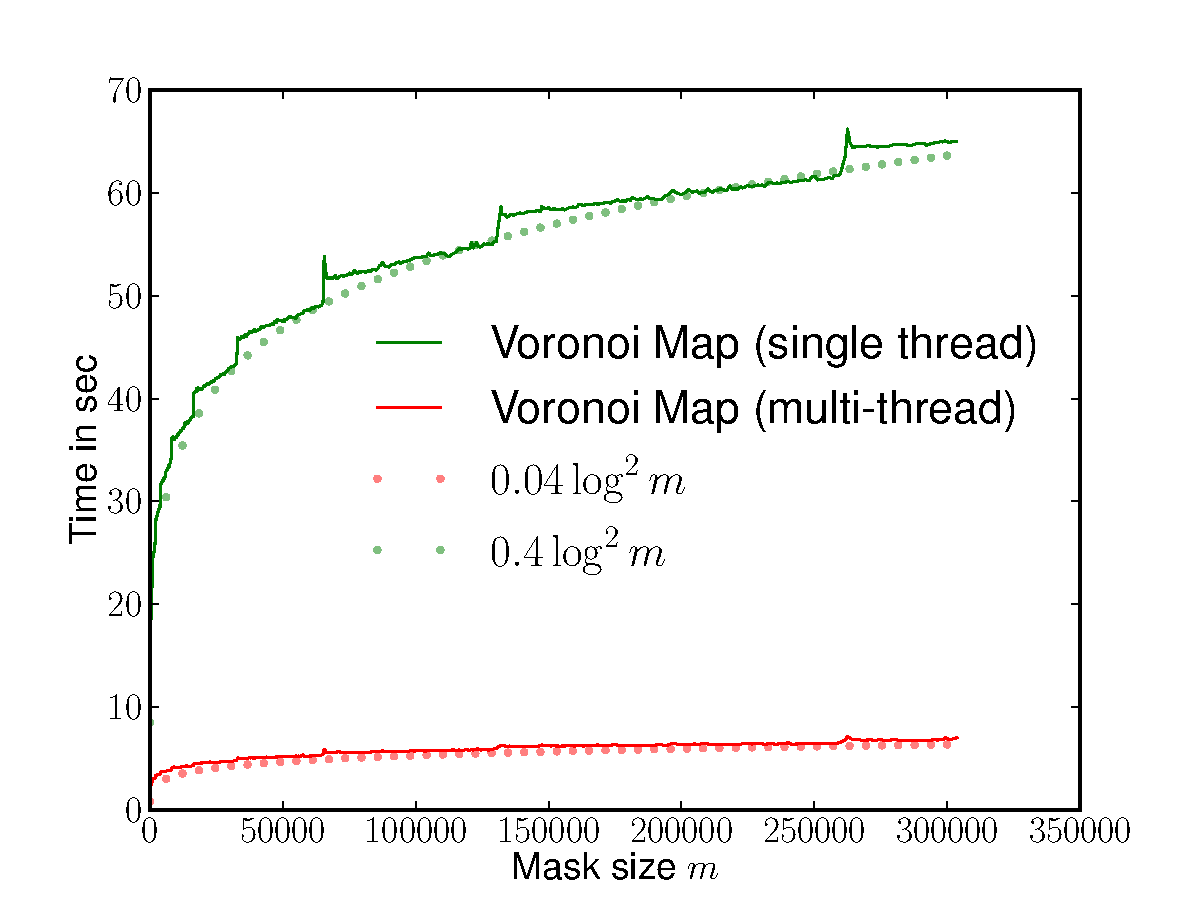
\includegraphics[origin=b,width=5.6cm]{data/result}}
    \end{tabular}
  \end{center}
  \caption{$(a)$ Separable Voronoi map and distance transformation for $\M_{5-7-11}$
    and $L_2$: on a $256^2$ domain with $256$ and $2$ random seeds,
    the first row corresponds to $\M_{5-7-11}$ and the second one to
    $L_2$. $(b)$ Experimental evaluation of subquadratic chamfer norm
    Voronoi map computation.  \label{fig:2Dvoro}}
\end{figure}
To evaluate experimentally the computational cost given in
Theorem~\ref{them}, we use the following setting: given a mask size
$m$, we generate $m$ distinct random vectors $(x,y)^T$ with
$gcd(x,y)=1$ (extracted from Farey series for instance). For a general
mask of size $m$, we do not optimize the weights to approximate as
best as possible the Euclidean metric. Indeed, weights do not play any
role in the computational analysis, we just use trivial ones that
ensure that $\M$ is a norm with axis symmetric unit ball.
In Fig.\ref{fig:2Dvoro}-$(b)$, we have considered a 2D domain $2048^2$
with $2048$ random sites. First, we observe that fixing $N$, the
$\log^2{m}$ term is clearly visible in the computational cost of the
Voronoi map (single thread curve). Bumps in the single thread curve
may be due to memory cache issues. Please note that if we consider
classical chamfer norm DT from raster scan (and half-masks), the
computational cost would have been in $O(m\cdot N^2)$ and thus would
have a linear behavior in Fig.~\ref{fig:2Dvoro}-$(b)$. Since we have a
separable algorithm, we can trivially implement it in a multi-thread
environment. Hence, on a bi-processor and quad-core (hyper-threading)
Intel(R) Xeon(R) cpu (16 threads can run in parallel), we observe a
speed-up by a factor 10 (blue curve in Fig.~\ref{fig:2Dvoro}-$(b)$).  Please
note that on this $2048^2$ domain with 2048 sites, Euclidean Voronoi
Map ($L_2$) is obtained in 954.837 milliseconds on a single core and
723.196 msec on 16 cores.

\section{Conclusion and Discussion}
\label{sec:discussion}

In the literature, several authors discussed about the fact that a
large class of metrics can be considered in separable approaches for
volumetric analysis. In this article, we have proposed several
algorithms to efficiently solve the Voronoi map and distance
transformation: given a user-specified distance function (induced by a
norm with some properties) a first generic separable algorithm can be
used. Focusing to chamfer norms, geometrical interpretation of this
generic approach allows us to design a first subquadratic algorithm in
dimension 2 to compute the Voronoi map.  \sloppy In higher dimensions,
it turns out that most results are still true: distance function can
be evaluated in $O(n\cdot\log{m})$ and the dichotomic search described
in \textsc{VoronoiEdgeWedge} can also be extended to $n$-dimensional
chamfer norms.



\bibliographystyle{splncs}
\bibliography{library,mybiblio,dtbib}
\end{document}
